\documentclass[tikz,border=0.12in]{standalone}
\usepackage{tikz}
\usepackage{amssymb}
\usepackage{fontawesome5}
\usetikzlibrary{positioning, arrows.meta, fit, backgrounds, calc}
\usepackage[T1]{fontenc}
\usepackage[scaled=0.95]{helvet}
\renewcommand{\familydefault}{\sfdefault}

\definecolor{miamired}{HTML}{C3142D}   % commercial / Miami / structure
\definecolor{pubgreen}{HTML}{2E7D5B}   % open public-good track
\definecolor{fundblue}{HTML}{2F5EA8}   % funded partners
\definecolor{nonfund}{HTML}{B8B49A}    % advisors / design partners
\definecolor{cornhusk}{HTML}{EFDB72}   % adjacent, beyond BWC scope

\tikzset{
  axisline/.style = {draw=gray!70, thick, -{Stealth[length=2.5mm]}},
  grid/.style     = {draw=gray!25, very thin},
  tick/.style     = {font=\scriptsize\bfseries, text=gray!60},
  grouplab/.style = {font=\footnotesize\bfseries, align=right, text width=2.8cm, text=black!80},
  groupbox/.style = {draw=black!45, thick, dashed, rounded corners},
  bandopen/.style = {rectangle, rounded corners, draw=pubgreen, ultra thick, fill=pubgreen!10,
                     align=left, font=\scriptsize, inner sep=5pt, text width=13.6cm, minimum height=0.85cm},
  bandcom/.style  = {rectangle, rounded corners, draw=miamired, ultra thick, fill=miamired!6,
                     align=left, font=\scriptsize, inner sep=5pt, text width=13.6cm, minimum height=0.85cm},
  wideband/.style = {rectangle, rounded corners, draw=nonfund!80!black, thick, fill=nonfund!30,
                     align=left, font=\scriptsize, inner sep=5pt, text width=13.6cm, minimum height=0.7cm},
  adjband/.style  = {rectangle, rounded corners, draw=cornhusk!70!black, ultra thick, dashed, fill=cornhusk!40,
                     align=left, font=\scriptsize, inner sep=5pt, text width=13.6cm, minimum height=0.7cm},
  ms/.style       = {rectangle, rounded corners=2pt, thick, align=center, text width=2.9cm,
                     font=\scriptsize, inner sep=3pt, minimum height=0.9cm},
  msF/.style      = {ms, draw=fundblue, fill=fundblue!7},
  msN/.style      = {ms, draw=nonfund!80!black, fill=nonfund!30},
  msR/.style      = {ms, draw=miamired, fill=miamired!6},
  ongoing/.style  = {draw=black!70, thick, -{Stealth[length=2.5mm]}, dash pattern=on 4pt off 2pt},
  terminus/.style = {rectangle, rounded corners, draw=miamired, ultra thick, fill=miamired!14,
                     align=center, font=\small, inner sep=5pt, text width=2.9cm, minimum height=3.8cm},
  conv/.style     = {draw=black, thick, -{Stealth[length=2.8mm]}},
}
\newcommand{\who}[1]{\textbf{#1:}~}

\begin{document}
\begin{tikzpicture}

% date x-positions: Jul25=0.6 Nov25=3.3 Mar26=6.2 Jun26=8.6 Dec26=11.2 Jun27=13.9
% --- faint gridlines ---
\foreach \x in {0.6,3.3,6.2,8.6,11.2,13.9} \draw[grid] (\x,8.05) -- (\x,-0.3);

% --- legend ---
\node [font=\scriptsize, anchor=west] at (-4.05,8.95) {%
  \textcolor{pubgreen}{$\blacksquare$}~Open (public good)\quad
  \textcolor{miamired}{$\blacksquare$}~Commercial / Miami\quad
  \textcolor{fundblue}{$\blacksquare$}~Funded partner\quad
  {\color{nonfund!80!black}$\blacksquare$}~Advisor\quad
  {\color{cornhusk!75!black}$\blacksquare$}~Adjacent (beyond BWC scope)};

% --- time axis ---
\draw[axisline] (0.2,8.3) -- (14.4,8.3);
\foreach \x/\lab in {0.6/{Jul '25},3.3/{Nov '25},6.2/{Mar '26},8.6/{Jun '26},11.2/{Dec '26},13.9/{Jun '27}}{
  \draw[gray!70] (\x,8.22) -- (\x,8.38);
  \node[tick, anchor=south] at (\x,8.44) {\lab};
}

% ===== GROUP A: overarching strategy (offerings) =====
\node (bopen) [bandopen, anchor=west] at (-1.1,6.6) {%
  \who{Open (public good \& strategic showcase)} web-based VR platform, open by design; builds visibility and seeds demand. \textit{Audience: workforce, educators, public.}};
\node (bcom) [bandcom, anchor=west] at (-1.1,5.5) {%
  \who{Commercial (licensable portfolio)} AR guidance $\cdot$ two-way cognitive digital twin $\cdot$ IIoT \textnormal{(enabling: computer vision, no IP)}. \textit{Audience: Ohio manufacturers. Model: licensing + joint development.}};
% sightvr.org public launch marker on the open band at Jun '26
\draw[pubgreen, thick] (8.6,7.02) -- (8.6,7.2);
\node[circle, fill=pubgreen, draw=white, line width=0.4pt, inner sep=1.6pt] at (8.6,7.02) {};
\node[anchor=south, font=\scriptsize\bfseries, text=pubgreen!80!black] at (8.6,7.2) {\faGlobe~sightvr.org public launch \textperiodcentered\ Jun 30, 2026};
\draw[groupbox] (-1.35,4.9) rectangle (13.4,7.7);
\node[grouplab] at (-2.85,5.9) {Overarching\\ strategy};

% ===== GROUP B: partner-led execution & IP =====
\node (mAR)   [msF] at (2.3,3.78) {\who{MaxByte} supports the AR build; interested in licensing our image-to-3D IP};
\node (mDisc) [msR] at (6.2,3.78) {\who{IP protection} two invention disclosures filed; in review ahead of a provisional patent};
\node (mHand) [msF] at (9.7,3.78) {\who{MeetKai} built the web-based VR platform; transferred to Miami hosting};
\draw[groupbox] (-1.35,2.9) rectangle (13.4,4.65);
\node[grouplab] at (-2.85,3.78) {Partner-led\\ execution \& IP};

% ===== GROUP C: market validation =====
\node (mOSC)  [msN] at (6.2,1.8) {OSC 2026 (20+ orgs) + FSB Advisory Council};
\node (mPilot)[msR] at (11.2,1.8) {\who{Pilot testing} usability validation \& optimization with industry + AM students (Task 5.1)};
\node (bDP) [wideband, anchor=west] at (-1.1,0.4) {%
  \who{Design partners} Yamaha, Engineered Profiles, Industrious Group: consulted on initial designs and iterative refinements};
\draw[groupbox] (-1.35,-0.3) rectangle (13.4,2.6);
\node[grouplab] at (-2.85,1.15) {Market validation};

% --- ongoing outreach & awareness ---
\draw[ongoing] (0.6,-0.95) -- (12.4,-0.95)
  node[midway, below=1pt, font=\scriptsize, text=black!70]
  {Ongoing outreach \& awareness since Jul '25:~~\faRss~blog~~~\faLinkedin~LinkedIn~~~\faChalkboardTeacher~seminars~~~and more};

% --- adjacent band (full timeline width, cornhusker yellow) ---
\node (adj) [adjband, anchor=west] at (-1.1,-1.9) {%
  \who{Adjacent (beyond BWC scope)} outside, non-BWC funding, e.g.\ a Department of Energy proposal with Yamaha applying the digital twin to energy management (see \S11)};

% ===== convergence terminus: the roadmap deliverable =====
\node (road) [terminus] at (15.9,3.7) {\textbf{Commercialization roadmap}\\[3pt]
  {\normalfont\scriptsize full, detailed roadmap delivered in Task 5.3 by Jun 30, 2027}};
\draw[conv] (13.4,6.3) to[out=0,in=145] (road.north west);
\draw[conv] (13.4,3.78) -- (road.west);
\draw[conv] (13.4,1.15) to[out=0,in=215] (road.south west);

\end{tikzpicture}
\end{document}
